%=======================================================================
%  An enthalpy formulation for latent heat storage in finned wellbore
%  heat exchangers, with branchwise-exact time integration.
%
%  Manuscript draft. Elsevier elsarticle class (preprint layout).
%  Companion project report: P2H2P_wellbore_TES (Overleaf).
%=======================================================================
\documentclass[preprint,12pt]{elsarticle}

\usepackage[T1]{fontenc}
\usepackage{amsmath,amssymb}
\usepackage{mathtools}
\usepackage{booktabs}
\usepackage{multirow}
\usepackage{longtable}
\usepackage{array}
\usepackage{siunitx}
\usepackage{graphicx}
\usepackage{xcolor}
\usepackage{enumitem}
\usepackage{tikz}
\usepackage{pgfplots}
\pgfplotsset{compat=1.18}
\usetikzlibrary{arrows.meta,positioning,calc}

\sisetup{per-mode=symbol}
\providecommand{\celsius}{\degreeCelsius}

% ---------- symbols ----------
\newcommand{\md}{\ensuremath{\dot m}}
\newcommand{\Ui}{\ensuremath{U_{i}}}
\newcommand{\hm}{\ensuremath{h_{m}}}
\newcommand{\Tm}{\ensuremath{T_{m}}}
\newcommand{\km}{\ensuremath{k_{m}}}
\newcommand{\rhom}{\ensuremath{\rho_{m}}}
\newcommand{\Amelt}{\ensuremath{A_{\mathrm{melt}}}}
\newcommand{\Aav}{\ensuremath{A_{\mathrm{avail}}}}
\newcommand{\Vmelt}{\ensuremath{V_{\mathrm{melt}}}}
\newcommand{\Nwells}{\ensuremath{N_{\mathrm{wells}}}}
\newcommand{\etao}{\ensuremath{\eta_{o}}}
\newcommand{\etaf}{\ensuremath{\eta_{f}}}
\newcommand{\Tpcm}{\ensuremath{T_{\mathrm{pcm}}}}
\newcommand{\Elat}{\ensuremath{E'_{\mathrm{lat}}}}
\newcommand{\Eeq}{\ensuremath{E'_{\mathrm{eq}}}}

\journal{Preprint}

\begin{document}

\begin{frontmatter}

\title{An enthalpy formulation for latent heat storage in finned tube
heat exchangers, with branchwise-exact time integration}

\author[lsu]{J.~R.~Barbosa~Jr.\corref{cor1}}
\ead{jrb@polo.ufsc.br}
\cortext[cor1]{Corresponding author.}

\address[lsu]{Craft \& Hawkins Department of Petroleum Engineering,
Louisiana State University, Baton Rouge, LA, USA}

\begin{abstract}
Reduced-order models of latent heat thermal energy storage commonly advance the
melt front as an \emph{area} or a \emph{thickness}, driven by the heat that a
resistance network delivers. Such a state variable cannot represent a control
volume whose phase change is complete: the model must either melt material that
is not there, or discard the delivered heat and break its own energy balance. In
a finned tube exchanger with an axially graded melting temperature the second
failure is not marginal --- in the case examined here the discarded heat reaches
\SI{148}{\percent} of the heat delivered during discharge.

This paper formulates the segment state as an \emph{enthalpy} per unit tube
length measured from a fully-solid datum, so that subcooled solid, two-phase and
superheated liquid are three branches of one single-valued curve and the melted
fraction is confined to $[0,1]$ by construction rather than by a guard. The
segment equation is derived from energy balances on the phase-change material
and on the fluid, and the closing conductance is shown to be
$K=\md c_{p}(1-e^{-\mathrm{NTU}})/\Delta z$ rather than the overall coefficient
times the perimeter; the two differ by up to \SI{33}{\percent} in the case
studied, and only the former carries the capacity-rate limit that prevents heat
flowing from cold to hot as the wall conductance improves.

The resulting equation is nonlinear but affine within each branch. A
branchwise-exact integrator is presented that solves each branch in closed form
and splits the step at branch crossings. It is unconditionally stable, preserves
energy closure to machine precision by construction, and agrees with a
\num{200000}-substep explicit reference to $3\times10^{-13}$. Explicit stepping
is shown to be inadmissible once sensible capacity is present, although it is
exact on the latent plateau --- which is why area-based formulations never
exposed the constraint.

The formulation is demonstrated on a phase-change material packed into the
annulus of a repurposed oil-and-gas well. Sensible capacity proves to be
self-levelling: a control volume that finishes melting begins to superheat, its
driving temperature difference collapses, and the heat passes downstream.
Compared at equal exchanger size, the spread in local melt fraction falls from
$0.405$ to $0.000$, and the phase-change material that never cycles --- dead
volume, carrying no energy through the round trip --- falls correspondingly.

Finally, the formulation is carried through repeated cycles to a cyclic steady
state. Because the state returns to itself and the store is adiabatic, the
ratio of recovered to stored energy is identically unity at cyclic steady
state, which removes the freedom that a single-cycle energy balance uses to
size the exchanger. The sizing problem is therefore reformulated as a
simulation: the hardware is specified, the cycle is marched to convergence, and
the deviation of delivered energy from target is reported as a result rather
than driven to zero.
\end{abstract}

\begin{keyword}
latent heat storage \sep phase change material \sep enthalpy method \sep
finned tube heat exchanger \sep effectiveness--NTU \sep exponential integrator
\end{keyword}

\end{frontmatter}

%=======================================================================
\section{Introduction}
\label{sec:intro}

Latent heat thermal energy storage couples a heat transfer fluid to a
phase-change material (PCM) through a wall, and the engineering problem is
almost always the same: the PCM conducts poorly, so the exchanger is finned,
staged, or otherwise elaborated until the phase change can be driven at the
required rate. Designing such an exchanger requires a model that couples a
\emph{heat transfer network} --- convection, wall, fins, and a growing melt
layer --- to a \emph{moving phase boundary}, over a duty cycle, at a cost low
enough to permit parametric study.

Two families of reduced-order model are in common use. Closed-form Stefan
solutions give the front position directly from a prescribed surface
temperature, and are attractive because they are explicit. Energy-balance
formulations instead advance the front from the heat that the network actually
delivers, which enforces conservation between the two sides of the wall. This
paper is concerned with a defect shared by both, and with what has to change to
remove it.

\subsection{The state variable, and what it cannot say}

Both families carry the melt front as a geometric quantity: a layer thickness
$\delta$, or equivalently a melted cross-sectional area $\Amelt$. Ask such a
model for the temperature of the PCM in a given control volume and the only
answer available is the melting temperature $\Tm$, because that is all the state
encodes. While solid remains, the answer is correct, which is why the limitation
is easy to miss.

It stops being correct the moment a control volume completes its phase change.
The network still reports a positive heat flow --- the fluid is still hotter
than $\Tm$, and nothing in the resistance chain knows the PCM is exhausted ---
and the model must do one of two things:

\begin{enumerate}[leftmargin=1.8em,itemsep=2pt]
\item \textbf{Continue melting.} $\Amelt$ grows past the PCM the control volume
  contains. Latent heat is drawn from material that is not there, and local
  melted fractions exceed unity.
\item \textbf{Clip and discard.} Cap $\Amelt$ at the available inventory and
  throw the surplus away. The melted fraction is then physical, but energy is
  not conserved, and the fluid leaves at a temperature that reflects heat which
  went nowhere.
\end{enumerate}

Neither is acceptable, and no refinement of the marching scheme repairs either,
because the deficiency is in the state: a variable counting melted area has no
slot for liquid above $\Tm$ or solid below it. The remedy adopted here is to
integrate enthalpy and recover the melted area from it --- the classical
enthalpy method \cite{Voller1987,Alexiades1993}, applied not to a discretised
field but to the lumped state of a one-dimensional exchanger segment.

\subsection{Contribution}

This paper makes three contributions, all concerning the formulation and its
numerics rather than the application:

\begin{enumerate}[leftmargin=1.8em,itemsep=3pt]
\item \textbf{A lumped enthalpy state for exchanger segments}
  (\S\ref{sec:formulation}). One scalar per segment encodes subcooled solid,
  two-phase and superheated liquid; the melted fraction is confined to $[0,1]$
  by the constitutive relation rather than by a guard, and no heat is ever
  discarded.
\item \textbf{The correct closing conductance} (\S\ref{sec:closure}). Deriving
  the segment equation from control-volume balances yields
  $K=\md c_{p}(1-e^{-\mathrm{NTU}})/\Delta z$, not $\Ui P_{i}$. The two agree
  only as $\mathrm{NTU}\to0$; the naive form lacks the capacity-rate limit and
  therefore permits unphysical behaviour as the wall conductance improves.
\item \textbf{A branchwise-exact integrator} (\S\ref{sec:integration}).
  Explicit stepping is exact on the latent plateau and inadmissible off it. The
  scheme presented solves each branch in closed form, splits steps at branch
  crossings, is unconditionally stable, and makes energy closure structural.
\end{enumerate}

\noindent
Section~\ref{sec:demo} demonstrates the formulation on a PCM-filled wellbore
heat exchanger and reports the physical consequence that motivated the work: the
self-levelling of the melt distribution.

%=======================================================================
\section{Enthalpy formulation}
\label{sec:formulation}

\subsection{Configuration and hypotheses}

Consider a tube of developed length $L_{\mathrm{tube}}$ carrying a
single-phase fluid at mass flow $\md$, surrounded by PCM. The tube is divided
into $n_{s}$ segments of length $\Delta z$ along the developed coordinate $s$.
Each segment owns a PCM cross-section $\Aav$, and the melting temperature may
vary from segment to segment, permitting an axially graded (cascaded) store in
which $\Tm$ follows the fluid glide.

The following are assumed throughout.

\begin{description}[leftmargin=1.9em,itemsep=2pt]
\item[H1] Quasi-steady conduction in the melt layer: its temperature profile is
  the steady cylindrical profile for the instantaneous front position. The
  hypothesis is controlled by the Stefan number
  $\mathrm{Ste}=c_{p}\Delta T/\hm$.
\item[H2] No axial conduction in the wall or the PCM; segments couple only
  through the fluid stream.
\item[H3] The melt region is a concentric annulus of uniform thickness $\delta$
  about each tube, and fronts about neighbouring tubes do not interact.
\item[H4] Conduction only in the melt; no natural convection in the liquid PCM.
\item[H5] One PCM temperature per segment: the state is lumped, with no radial
  resolution of temperature \emph{within} a phase.
\item[H6] Adiabatic outer boundary.
\item[H7] Incompressible single-phase fluid, treated as quasi-steady.
\end{description}

\subsection{Why enthalpy rather than temperature}

The natural repair for the deficiency of \S\ref{sec:intro} is to carry a PCM
temperature alongside the melted area. It is the wrong repair, for a reason that
recurs throughout phase-change modelling: at a phase change, temperature is not
invertible. During melting the PCM remains at $\Tm$ while its energy content
climbs by the entire latent heat, so $T$ carries no information whatever
throughout the process that dominates the problem. A pair $(T,\Amelt)$ works,
but obliges the code to decide at every step which member is active, keep the
two consistent, and handle the instants at which the active member changes.

Enthalpy is invertible. Every state of the PCM corresponds to exactly one value
of the enthalpy, and the enthalpy increases monotonically as heat is added. A
single scalar per segment therefore encodes all three regimes, and the regime is
read from the value rather than tracked separately
(Fig.~\ref{fig:enthalpy-curve}).

\begin{figure}[htbp]
\centering
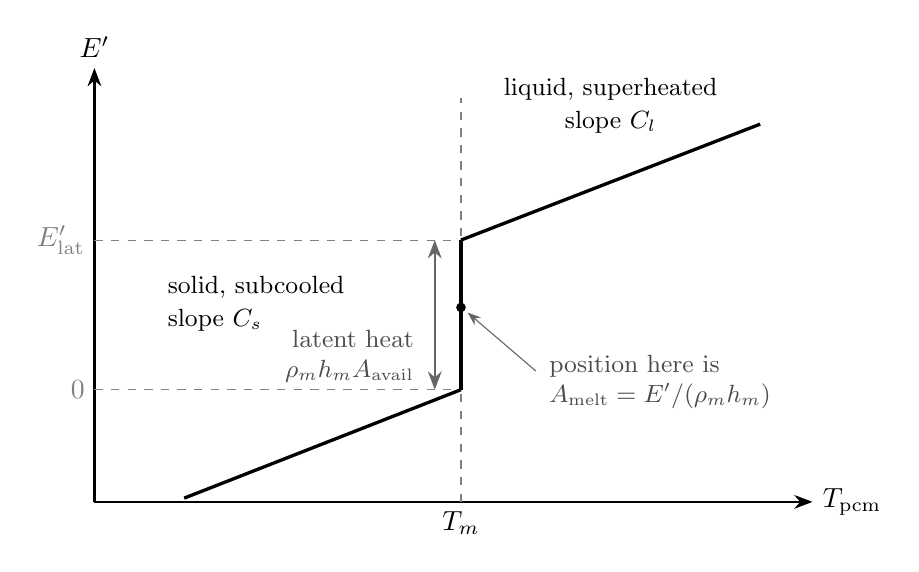
\begin{tikzpicture}[>=Stealth, scale=0.95]
  \draw[->,thick] (0,0) -- (9.6,0) node[right] {$\Tpcm$};
  \draw[->,thick] (0,0) -- (0,5.8) node[above] {$E'$};
  \draw[dashed,gray] (4.9,0) -- (4.9,5.4);
  \node[below] at (4.9,0) {$\Tm$};
  \draw[dashed,gray] (0,1.5) -- (4.9,1.5) node[pos=0,left] {$0$};
  \draw[dashed,gray] (0,3.5) -- (4.9,3.5) node[pos=0,left] {$\Elat$};
  \draw[very thick] (1.2,0.05) -- (4.9,1.5);
  \draw[very thick] (4.9,1.5) -- (4.9,3.5);
  \draw[very thick] (4.9,3.5) -- (8.9,5.05);
  \node[align=left,font=\small,anchor=west] at (0.85,2.65)
    {solid, subcooled\\[1pt] slope $C_{s}$};
  \node[align=center,font=\small] at (6.9,5.3)
    {liquid, superheated\\[1pt] slope $C_{l}$};
  \draw[<->,thick,black!60] (4.55,1.5) -- (4.55,3.5);
  \node[font=\small,align=right,anchor=east,black!70] at (4.4,1.95)
    {latent heat\\$\rhom\hm\Aav$};
  \filldraw (4.9,2.6) circle (1.6pt);
  \draw[->,black!60] (5.9,1.75) -- (4.99,2.53);
  \node[font=\small,align=left,anchor=west,black!70] at (5.95,1.6)
    {position here is\\$\Amelt = E'/(\rhom\hm)$};
\end{tikzpicture}
\caption{The constitutive curve, Eq.~\eqref{eq:enth-curve}. Read as $E'(T)$ it
is multivalued at $\Tm$, which is why temperature cannot serve as the state.
Read as $T(E')$ --- the direction used here --- it is single-valued everywhere,
and position along the vertical segment is the melted fraction.}
\label{fig:enthalpy-curve}
\end{figure}

\subsection{State and capacities}

Let $E'$ be the enthalpy per unit tube length of the PCM belonging to one
segment, measured from a datum of fully solid material at $\Tm$. The datum is
arbitrary; this choice places the two branch boundaries at $0$ and $\Elat$,
which shortens every test in the implementation. With
\begin{equation}
  \Elat = \rhom\hm\Aav,
  \qquad
  C_{s} = \rhom c_{p,s}\Aav,
  \qquad
  C_{l} = \rhom c_{p,l}\Aav,
  \label{eq:caps}
\end{equation}
the latent capacity and the two sensible capacities per unit tube length, the
constitutive curve and the melted area are
\begin{equation}
  \Tpcm =
  \begin{dcases}
    \Tm + E'/C_{s}, & E' < 0 \quad\text{(solid, subcooled)},\\[2pt]
    \Tm, & 0 \le E' \le \Elat \quad\text{(two-phase)},\\[2pt]
    \Tm + \bigl(E'-\Elat\bigr)/C_{l},
      & E' > \Elat \quad\text{(liquid, superheated)},
  \end{dcases}
  \label{eq:enth-curve}
\end{equation}
\begin{equation}
  \Amelt = \frac{\min\!\bigl(\max(E',0),\,\Elat\bigr)}{\rhom\hm},
  \qquad
  \varepsilon_{\mathrm{local}} = \frac{\Amelt}{\Aav} \in [0,1].
  \label{eq:amelt}
\end{equation}

The saturation in Eq.~\eqref{eq:amelt} is not a guard added to suppress bad
behaviour; it is the definition. Melted area saturates because a segment cannot
melt PCM it does not own, and superheat is where the additional energy goes.
Consequently $\varepsilon_{\mathrm{local}}\in[0,1]$ is \emph{structural}: no
code path can violate it, and no test for it is required.

\subsection{Recovering the layer thickness}

The resistance network requires $\delta$, not $\Amelt$. For a tube of outer
radius $r_{e}$ carrying $n_{f}$ longitudinal fins of thickness $t_{f}$ and
radial length $L_{f}$, the fin metal occupies part of the annulus and must be
excluded from the melted PCM area:
\begin{equation}
  \Amelt = \pi\left[(r_{e}+\delta)^{2}-r_{e}^{2}\right]
           - n_{f}t_{f}\min\!\left(\delta,L_{f}\right),
  \label{eq:area-fins}
\end{equation}
which inverts in closed form on each branch,
\begin{align}
  \delta \le L_{f}: &\quad
    \pi\delta^{2}+\left(2\pi r_{e}-n_{f}t_{f}\right)\delta-\Amelt = 0,
  \label{eq:delta-in}\\
  \delta > L_{f}: &\quad
    \pi\delta^{2}+2\pi r_{e}\delta-\left(\Amelt+n_{f}t_{f}L_{f}\right) = 0 .
  \label{eq:delta-out}
\end{align}
For $n_{f}=0$ both reduce to
$\delta=\sqrt{r_{e}^{2}+\Amelt/\pi}-r_{e}$.

The melt layer then enters the network as a cylindrical conduction shell,
\begin{equation}
  h_{e} = \frac{\km}{r_{e}\ln\!\left(1+\delta/r_{e}\right)},
  \label{eq:he}
\end{equation}
and the overall coefficient on the inner area, with fin efficiency $\etaf$,
overall surface efficiency $\etao$ and finned perimeter $P_{T}$, is
\begin{equation}
  \Ui = \left[\frac{1}{h_{i}} + R''_{f,i}
        + \frac{r_{i}}{k_{w}}\ln\frac{r_{e}}{r_{i}}
        + \frac{2\pi r_{i}}{P_{T}\,\etao\,h_{e}}\right]^{-1}.
  \label{eq:Ui}
\end{equation}

The single change relative to an area-based formulation is that the outer
boundary of this chain sits at $\Tpcm$, not at $\Tm$. It coincides with $\Tm$
only while solid remains. Section~\ref{sec:demo} shows that this one
substitution is responsible for the principal physical result.

%=======================================================================
\section{The segment equation and its closure}
\label{sec:closure}

Equation~\eqref{eq:ode} below is short enough to look like a definition. It is
not: it follows from energy balances on two control volumes and the elimination
of the quantity they share. The derivation is given in full because the closing
conductance is not the one a reader would write down unaided.

\subsection{Two control volumes}

Fix a segment $j$ spanning $s\in[s_{j},s_{j+1}]$, $\Delta z=s_{j+1}-s_{j}$. Two
control volumes share the tube wall over that interval: \textbf{CV\,1}, the PCM
belonging to the segment --- cross-section $\Aav$, stationary, closed --- and
\textbf{CV\,2}, the fluid within the tube over the same interval, open, entering
at $T_{j}$ and leaving at $T_{j+1}$. Write $q'_{j}$ for the heat per unit tube
length crossing from CV\,2 into CV\,1.

\subsection{The PCM balance}

CV\,1 is closed and stationary, so the first law reduces to a statement about
its enthalpy. With the axial (H2) and outer-boundary (H6) terms dropped,
\begin{equation}
  \boxed{\;\frac{\mathrm{d}E'_{j}}{\mathrm{d}t} = q'_{j}\;}
  \label{eq:pcm-balance}
\end{equation}

\subsection{The fluid balance}

For incompressible single-phase flow without viscous dissipation, the energy
equation per unit tube length is
\begin{equation}
  \rho A_{\mathrm{flow}} c_{p}\frac{\partial T}{\partial t}
  + \md c_{p}\frac{\partial T}{\partial s} = -q'(s).
  \label{eq:fluid-pde}
\end{equation}
Hypothesis H7 drops the first term. The approximation is justified by the
separation between the fluid transit time and the timescale of the PCM state,
and its cost is an unresolved startup transient of one transit at the beginning
of each half-cycle; \S\ref{sec:demo} quantifies both for the case studied.

With CV\,1 presenting a single temperature to the whole segment (H5), the local
flux closes on the network,
\begin{equation}
  q'(s) = \Ui\,(2\pi r_{i})\left[T(s)-\Tpcm\right].
  \label{eq:local-flux}
\end{equation}
The inner perimeter $2\pi r_{i}$ appears rather than $P_{T}$ because $\Ui$ was
referred to the inner area in Eq.~\eqref{eq:Ui}; the finned perimeter is already
inside it. Using $P_{T}$ here would count the fins twice.

\subsection{Integration across the segment}

Substituting Eq.~\eqref{eq:local-flux} into the steady form of
Eq.~\eqref{eq:fluid-pde}, with $\Tpcm$ and $\Ui$ held constant over the segment,
gives a linear ordinary differential equation in $s$ whose solution is the
single-stream heat exchanger result:
\begin{equation}
  T_{j+1} = \Tpcm + \left(T_{j}-\Tpcm\right)e^{-\mathrm{NTU}_{j}},
  \qquad
  \mathrm{NTU}_{j} = \frac{2\pi r_{i}\,\Ui\,\Delta z}{\md\,c_{p}}.
  \label{eq:ntu}
\end{equation}
One stream carries a finite capacity rate $\md c_{p}$; the other is an
isothermal reservoir of infinite capacity rate, with effectiveness
$\varepsilon=1-e^{-\mathrm{NTU}}$. The reservoir idealisation is precisely what
the lumped state of H5 licenses.

\subsection{The closure, and why the conductance is not $\Ui P_{i}$}

The heat the fluid gives up over the segment is the enthalpy it loses, so from
Eq.~\eqref{eq:ntu},
\begin{equation}
  \boxed{\;
  q'_{j} = K_{j}\left(T_{j}-\Tpcm\right),
  \qquad
  K_{j} = \frac{\md c_{p}\left(1-e^{-\mathrm{NTU}_{j}}\right)}{\Delta z}.
  \;}
  \label{eq:K}
\end{equation}
Combining Eqs.~\eqref{eq:pcm-balance}, \eqref{eq:K} and \eqref{eq:enth-curve}
closes the system:
\begin{equation}
  \boxed{\;
  \frac{\mathrm{d}E'}{\mathrm{d}t}
  = K\left(T_{j}-\Tpcm(E')\right)
  \;}
  \label{eq:ode}
\end{equation}
with one unknown per segment; everything else is geometry, a property, or the
upstream fluid temperature handed down by the preceding segment.

The naive closure evaluates Eq.~\eqref{eq:local-flux} at $T(s)\approx T_{j}$,
giving $q'_{j}\approx 2\pi r_{i}\Ui(T_{j}-\Tpcm)$. Comparing,
\begin{equation}
  \frac{K_{j}}{2\pi r_{i}\Ui}
  = \frac{1-e^{-\mathrm{NTU}_{j}}}{\mathrm{NTU}_{j}} \le 1,
  \label{eq:K-ratio}
\end{equation}
and the two limits say what the difference means. As $\mathrm{NTU}\to0$ the
ratio tends to unity: the fluid barely cools across the segment and the naive
closure is correct. As $\mathrm{NTU}\to\infty$, $K\to\md c_{p}/\Delta z$, a
finite limit set by the \emph{fluid} rather than the wall --- a segment cannot
absorb more than the stream delivers to it. The naive closure has no such limit:
it permits $T_{j+1}$ to fall below $\Tpcm$, that is, heat flowing from cold to
hot, at a rate growing without bound as $\Ui$ improves. The discrepancy is
largest where the melt layer is thinnest and the exchanger best, which is where
the model is most active.

\subsection{Closure is structural}

Equation~\eqref{eq:K} is not evaluated independently of
Eq.~\eqref{eq:pcm-balance}. The implementation integrates
Eq.~\eqref{eq:pcm-balance} over the step and \emph{reports}
\begin{equation}
  q'_{j} = \frac{E'^{\,n+1}-E'^{\,n}}{\Delta t},
  \label{eq:qfromE}
\end{equation}
then drops the fluid temperature by exactly that amount,
$T_{j+1}=T_{j}-q'_{j}\Delta z/(\md c_{p})$. Whatever the PCM gained, the fluid
lost, to machine precision, with no possibility of drift. It should be stressed
that this is a \emph{consistency} property and not evidence of correctness: the
two operations are inverse, so a small residual measures floating-point
arithmetic and nothing else.

%=======================================================================
\section{Branchwise-exact time integration}
\label{sec:integration}

\subsection{Why explicit stepping is inadmissible}

Equation~\eqref{eq:ode} is nonlinear, because $\Tpcm(E')$ is piecewise, but
affine within each branch of Eq.~\eqref{eq:enth-curve}. The distinction governs
the choice of integrator.

On the latent plateau $\Tpcm=\Tm$ is constant and does not respond to $E'$ at
all. The segment behaves as though its heat capacity were infinite,
Eq.~\eqref{eq:ode} reduces to $\mathrm{d}E'/\mathrm{d}t=\text{const}$, and an
explicit Euler step is not merely stable but exact. This is the regime an
area-based formulation occupies permanently, which explains why the constraint
derived below has not previously been a concern: explicit stepping was safe for
a structural reason, not a fortunate one.

Introducing sensible capacity makes the capacity finite. Equation~\eqref{eq:ode}
becomes a relaxation equation with time constant $C/K$, and explicit Euler
requires $\Delta t < C/K$. Logarithmic time grids, which are the natural choice
for a diffusion-limited process, violate this at late times by a wide margin;
\S\ref{sec:demo} gives the figures for the case studied, where the final step
exceeds the limit by a factor of $7.7$ and an explicit implementation diverges.

\subsection{The scheme}

Rather than reduce $\Delta t$ --- which for a logarithmic grid multiplies the
cost by some three orders of magnitude --- the linearity within each branch is
exploited and each branch integrated in closed form. Holding $T_{j}$ fixed
across the step,
\begin{equation}
  E'(t+\Delta t) =
  \begin{dcases}
    E' + K\left(T_{j}-\Tm\right)\Delta t,
      & \text{plateau,}\\[4pt]
    \Eeq + \bigl(E'-\Eeq\bigr)e^{-K\Delta t/C},
      & \text{sensible branches,}
  \end{dcases}
  \label{eq:exact}
\end{equation}
with the equilibrium enthalpy and relevant capacity
\begin{equation}
  \left(C,\Eeq\right) =
  \begin{cases}
    \left(C_{s},\;C_{s}\left(T_{j}-\Tm\right)\right), & E'<0,\\[3pt]
    \left(C_{l},\;\Elat+C_{l}\left(T_{j}-\Tm\right)\right), & E'>\Elat.
  \end{cases}
  \label{eq:Eeq}
\end{equation}
$\Eeq$ is the enthalpy at which the PCM would sit in equilibrium with the fluid:
the state the segment relaxes toward and never reaches. The exponential is
unconditionally stable and monotone, so no step, however large, can overshoot
it. That is precisely the property explicit Euler lacks.

\subsection{Branch crossings}

A step may begin in one branch and end in another, in which case it is split at
the crossing. With $E'_{b}$ the boundary being approached ($0$ or $\Elat$), the
crossing time is
\begin{equation}
  t^{*} =
  \begin{dcases}
    \frac{E'_{b}-E'}{K\left(T_{j}-\Tm\right)}, & \text{from the plateau},\\[8pt]
    \frac{C}{K}\ln\!\left(\frac{E'-\Eeq}{E'_{b}-\Eeq}\right),
      & \text{from a sensible branch}.
  \end{dcases}
  \label{eq:crossing}
\end{equation}
If $t^{*}<\Delta t$ the state is advanced to $E'_{b}$, the remaining
$\Delta t-t^{*}$ is integrated in the adjacent branch, and the test repeated.
Only a small number of crossings can occur within one step, so the loop is
bounded.

\begin{table}[htbp]
\centering
\caption{Algorithm: advance one segment over $\Delta t$.}
\label{tab:algorithm}
\begin{tabular}{@{}r l@{}}
\toprule
 & \\[-8pt]
1 & $t_{\mathrm{left}} \leftarrow \Delta t$, \quad $E'_{0}\leftarrow E'$ \\
2 & \textbf{while} $t_{\mathrm{left}}>0$: \\
3 & \quad identify the branch containing $E'$ \\
4 & \quad compute $t^{*}$ from Eq.~\eqref{eq:crossing} toward the branch boundary \\
5 & \quad \textbf{if} $t^{*} \ge t_{\mathrm{left}}$: advance by Eq.~\eqref{eq:exact}
        over $t_{\mathrm{left}}$; \textbf{break} \\
6 & \quad \textbf{else}: set $E'\leftarrow E'_{b}\pm\epsilon$;\quad
        $t_{\mathrm{left}} \leftarrow t_{\mathrm{left}}-t^{*}$ \\
7 & \textbf{return} $E'$, \quad $q' = (E'-E'_{0})/\Delta t$ \\[2pt]
\bottomrule
\end{tabular}
\end{table}

\paragraph{A note on the boundary test.}
Step 6 of Table~\ref{tab:algorithm} displaces the state just past the boundary
by $\epsilon=10^{-9}\max(\Elat,1)$ rather than placing it exactly on the
boundary. This is necessary rather than cosmetic. If the branch test uses closed
intervals, a state landing exactly on $\Elat$ is still classified as two-phase;
the plateau branch then computes $t^{*}=0$, advances the state to where it
already is, subtracts zero from the remaining time, and repeats indefinitely.
The segment is pinned at the boundary and never enters the liquid branch. The
symptom is not a failure but an apparent success --- every segment reporting a
melted fraction of exactly unity and zero superheat. The general point is that
where a solver switches on the sign of a quantity, the side of the boundary to
which equality belongs must be chosen deliberately, and the state must not be
able to come to rest there.

%---------------------------------------------------------------------
\begin{figure}[htbp]
\centering
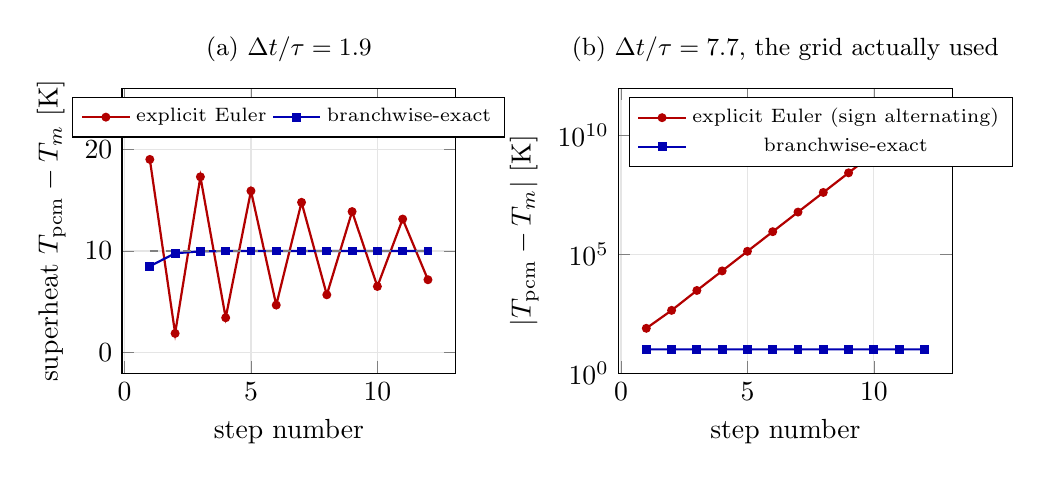
\begin{tikzpicture}
\begin{axis}[width=0.48\linewidth,height=5.2cm,
  xlabel={step number}, ylabel={superheat $\Tpcm-\Tm$ [K]},
  title={\small (a) $\Delta t/\tau=1.9$}, ymin=-2, ymax=26,
  legend style={font=\scriptsize,at={(0.5,0.97)},anchor=north},
  legend columns=2,
  grid=both, grid style={gray!20}]
\addplot[thick,mark=*,mark size=1.2pt,red!70!black] coordinates {(1,19.0) (2,1.9) (3,17.29) (4,3.439) (5,15.9049) (6,4.6856) (7,14.783) (8,5.6953) (9,13.8742) (10,6.5132) (11,13.1381) (12,7.1757)};
\addlegendentry{explicit Euler}
\addplot[thick,mark=square*,mark size=1.2pt,blue!70!black] coordinates {(1,8.5043) (2,9.7763) (3,9.9665) (4,9.995) (5,9.9993) (6,9.9999) (7,10.0) (8,10.0) (9,10.0) (10,10.0) (11,10.0) (12,10.0)};
\addlegendentry{branchwise-exact}
\addplot[dashed,gray,domain=1:12,forget plot] {10};
\end{axis}
\begin{axis}[width=0.48\linewidth,height=5.2cm,at={(0.52\linewidth,0)},
  xlabel={step number}, ylabel={$|\Tpcm-\Tm|$ [K]}, ymode=log,
  title={\small (b) $\Delta t/\tau=7.7$, the grid actually used},
  ymin=1, ymax=1e12, legend style={font=\scriptsize,at={(0.03,0.97)},anchor=north west},
  grid=both, grid style={gray!20}]
\addplot[thick,mark=*,mark size=1.2pt,red!70!black] coordinates {
  (1,77) (2,438.9) (3,3017.6) (4,20141) (5,135023) (6,904574)
  (7,6.0607e6) (8,4.0607e7) (9,2.7207e8) (10,1.8228e9) (11,1.2213e10) (12,8.1827e10)};
\addlegendentry{explicit Euler (sign alternating)}
\addplot[thick,mark=square*,mark size=1.2pt,blue!70!black] coordinates {
  (1,9.9955) (2,10) (3,10) (4,10) (5,10) (6,10) (7,10) (8,10) (9,10) (10,10) (11,10) (12,10)};
\addlegendentry{branchwise-exact}
\end{axis}
\end{tikzpicture}
\caption{Response of a single segment on the liquid branch, driven by fluid
\SI{10}{\kelvin} above $\Tm$ with $\tau=C_{l}/K=\SI{1102}{\second}$.
(a) At $\Delta t/\tau=1.9$ explicit Euler oscillates about the equilibrium
while remaining bounded. (b) At $\Delta t/\tau=7.7$ --- the ratio the
logarithmic grid of Table~\ref{tab:stability} actually reaches at the end of a
charge --- it diverges, alternating in sign and passing
\SI{8e10}{\kelvin} within twelve steps. The branchwise-exact scheme is
monotone and correct at every step size, because Eq.~\eqref{eq:exact} cannot
overshoot $\Eeq$.}
\label{fig:stability}
\end{figure}


%---------------------------------------------------------------------
\begin{figure}[htbp]
\centering
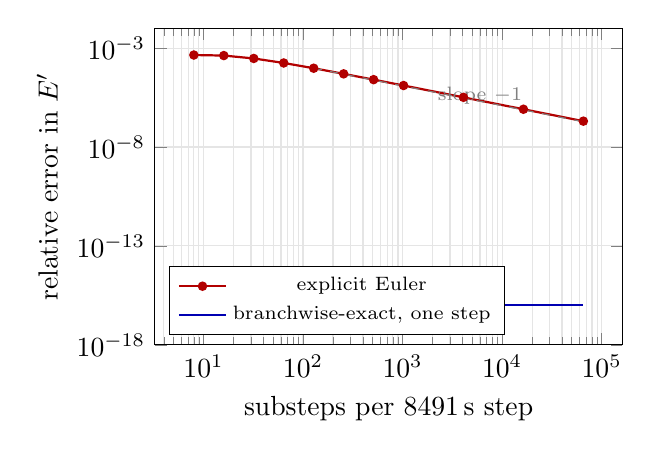
\begin{tikzpicture}
\begin{axis}[width=0.62\linewidth,height=5.6cm,
  xlabel={substeps per \SI{8491}{\second} step}, ylabel={relative error in $E'$},
  xmode=log, ymode=log, ymin=1e-18, ymax=1e-2,
  legend style={font=\scriptsize,at={(0.03,0.03)},anchor=south west},
  grid=both, grid style={gray!20}]
\addplot[thick,mark=*,mark size=1.3pt,red!70!black] coordinates {(8,4.4986e-4) (16,4.2272e-4) (32,3.0168e-4) (64,1.7837e-4) (128,9.6617e-5) (256,5.0229e-5) (512,2.5602e-5) (1024,1.2924e-5) (4096,3.2541e-6) (16384,8.1497e-7) (65536,2.0383e-7)};
\addlegendentry{explicit Euler}
\addplot[thick,blue!70!black,domain=8:65536,samples=2] {1e-16};
\addlegendentry{branchwise-exact, one step}
\addplot[dashed,gray,domain=128:65536,samples=2,forget plot] {1.24e-2/x};
\node[font=\scriptsize,gray] at (axis cs:6000,4e-6) {slope $-1$};
\end{axis}
\end{tikzpicture}
\caption{Error after advancing one segment through a single \SI{8491}{\second}
grid step, against the number of explicit substeps used. Explicit Euler is
first order once it is stable ($\ge 8$ substeps; below that it is not), and
needs of order $10^{4}$ substeps to reach $10^{-6}$. The branchwise-exact
scheme returns the closed-form solution of the branch, so its error is zero to
machine precision in a \emph{single} step --- plotted at $10^{-16}$ for
visibility.}
\label{fig:convergence}
\end{figure}


\subsection{Verification}
\label{sec:verification}

The scheme was verified against a brute-force explicit integration of
Eq.~\eqref{eq:ode} using \num{200000} substeps, over a complete charge and
discharge, including steps crossing branch boundaries. Agreement is
$3\times10^{-13}$ in relative terms, which is machine precision. The two
calculations share no code path beyond Eq.~\eqref{eq:enth-curve}, so this is a
genuine verification of the integrator rather than a consistency check.

Energy closure, by contrast, is structural under Eq.~\eqref{eq:qfromE} and
therefore proves nothing about correctness; it is reported here only to
establish that no drift is present.

%=======================================================================
\section{Demonstration: a PCM-filled wellbore heat exchanger}
\label{sec:demo}

\subsection{Configuration}

The formulation is demonstrated on latent heat storage in the annulus of a
repurposed oil-and-gas well. A high-temperature heat pump melts the PCM during
charging and an organic Rankine cycle recovers the energy during discharging,
with pressurised water circulating through finned hairpin tubes in the borehole.
Table~\ref{tab:config} gives the configuration.

\begin{table}[htbp]
\centering
\caption{Configuration of the demonstration case.}
\label{tab:config}
\begin{tabular}{@{}l l r l@{}}
\toprule
 & quantity & value & unit \\
\midrule
\multirow{4}{*}{Borehole}
 & depth $L_{\mathrm{well}}$ & 1524 & \si{\meter} \\
 & diameter $D_{\mathrm{well}}$ & 177.8 & \si{\milli\meter} \\
 & hairpin tubes $n_{t}$ & 2 & -- \\
 & PCM volume $V_{\mathrm{well}}$ & 27.68 & \si{\meter\cubed} \\
\midrule
\multirow{4}{*}{Tube}
 & inner radius $r_{i}$ & 16.23 & \si{\milli\meter} \\
 & outer radius $r_{e}$ & 21.08 & \si{\milli\meter} \\
 & fins per leg $n_{f}$ & 24 & -- \\
 & fin $L_{f}\times t_{f}$ & $7.5\times1.5$ & \si{\milli\meter} \\
\midrule
\multirow{5}{*}{PCM}
 & melting temperature $\Tm$ & 150 & \si{\celsius} \\
 & latent heat $\hm$ & 380 & \si{\kilo\joule\per\kilogram} \\
 & $c_{p,s}$ / $c_{p,l}$ & 1280 / 1800 & \si{\joule\per\kilogram\per\kelvin} \\
 & $k_{s}$ / $k_{l}$ & 0.60 / 0.45 & \si{\watt\per\meter\per\kelvin} \\
 & $\rho_{s}$ / $\rho_{l}$ & 1550 / 1450 & \si{\kilogram\per\meter\cubed} \\
\midrule
\multirow{4}{*}{Operation}
 & fluid glide $\Delta T_{3C,2C}$ & 55 & \si{\kelvin} \\
 & charging inlet & 160 & \si{\celsius} \\
 & charge / discharge window & 10 / 10 & \si{\hour} \\
 & PCM layers $N_{\mathrm{lay}}$ & 9 & -- \\
\bottomrule
\end{tabular}
\end{table}

\noindent
The resulting capacities, Eq.~\eqref{eq:caps}, are
$\Aav=\SI{4.5411e-3}{\meter\squared}$,
$\Elat=\SI{2.675}{\mega\joule\per\meter}$,
$C_{s}=\SI{9.010e3}{\joule\per\meter\per\kelvin}$ and
$C_{l}=\SI{1.267e4}{\joule\per\meter\per\kelvin}$. The ratio
$C_{l}/\Elat=\SI{4.74e-3}{\per\kelvin}$ is the Stefan number in disguise: one
kelvin of superheat is worth \SI{0.47}{\percent} of the latent capacity, so with
the \SI{10}{\kelvin} approach available here the sensible branches carry at most
about \SI{4.7}{\percent} of the energy. A reader might reasonably conclude that
the formulation is a small correction. Section~\ref{sec:levelling} shows why it
is not.

\subsection{Quasi-steady fluid: the cost of H7}

Table~\ref{tab:h7} collects the comparisons that justify dropping
$\partial T/\partial t$ from Eq.~\eqref{eq:fluid-pde}.

\begin{table}[htbp]
\centering
\caption{Justification and cost of the quasi-steady fluid approximation.}
\label{tab:h7}
\begin{tabular}{@{}l r l@{}}
\toprule
quantity & value & \\
\midrule
fluid transit time over $L_{\mathrm{tube}}$ & \SI{2264}{\second}
  & ($u=\SI{1.35}{\meter\per\second}$) \\
charging window $t_{\mathrm{ch}}$ & \SI{36000}{\second} & \\
ratio & \num{0.063} & \\
$\rho A_{\mathrm{flow}}c_{p}/C_{l}$ & \num{0.257}
  & fluid vs.\ PCM sensible capacity \\
$\rho A_{\mathrm{flow}}c_{p}\Delta T/\Elat$ & \num{0.0122}
  & fluid swing vs.\ latent, $\Delta T=\SI{10}{\kelvin}$ \\
\bottomrule
\end{tabular}
\end{table}

\noindent
The fluid re-establishes its profile in one transit while the PCM state evolves
over ten hours, a separation of about sixteen. The approximation is therefore
reasonable but not asymptotic: the first \SI{38}{\minute} of each half-cycle is
a startup transient the model does not resolve, some \SI{6}{\percent} of the
window. What renders this tolerable is the last row --- the energy held in the
fluid is only \SI{1.2}{\percent} of the latent inventory it is charging, so the
transient misplaces very little energy even though it occupies a noticeable
fraction of the run.

\subsection{The closure discrepancy in practice}

Over the charge, $\mathrm{NTU}$ ranges from \num{0.083} to \num{0.602}, so
Eq.~\eqref{eq:K-ratio} lies between \num{0.96} and \num{0.75}. Using
$\Ui P_{i}$ in place of Eq.~\eqref{eq:K} would therefore overstate the segment
conductance by between \SI{4}{\percent} and \SI{33}{\percent} in this case, with
the largest error at early times when the melt layer is thin and the exchanger
at its best.

\subsection{Stability of the time integration}

Table~\ref{tab:stability} gives the stability figures for the logarithmic time
grid used here.

\begin{table}[htbp]
\centering
\caption{Explicit-Euler stability limit against the time grid actually used,
for the first segment.}
\label{tab:stability}
\begin{tabular}{@{}l r r@{}}
\toprule
 & early ($t=\SI{1}{\second}$) & late ($t\to t_{\mathrm{ch}}$) \\
\midrule
$\mathrm{NTU}$ & \num{0.592} & \num{0.083} \\
$K$ [\si{\watt\per\meter\per\kelvin}] & \num{64.3} & \num{11.5} \\
$C_{l}/K$ [\si{\second}] & \num{197} & \num{1106} \\
grid step $\Delta t$ [\si{\second}] & \num{0.31} & \num{8491} \\
\midrule
$\Delta t\,K/C_{l}$ & \num{0.002} & \textbf{\num{7.7}} \\
\bottomrule
\end{tabular}
\end{table}

\noindent
The grid is comfortable at the start and violates the limit by almost an order
of magnitude at the end. An explicit implementation duly diverged, the
oscillation feeding back through the fluid temperature and driving the secondary
fluid to \SI{261}{\kelvin} --- some \SI{170}{\kelvin} below anything physical.
That failure was loud and immediately diagnosable; the dangerous case is a step
ratio nearer $1.5$, unstable in principle but slowly enough to resemble a
plausible answer.

\subsection{Sensible capacity is self-levelling}
\label{sec:levelling}

The principal physical result is not the magnitude of the sensible energy but
its effect on the \emph{distribution} of melting.

Consider the segment nearest the inlet, which sees the hottest fluid and
therefore melts first. Under an area-based formulation it finishes melting and
then continues to absorb heat at the full driving difference $T_{j}-\Tm$,
because its boundary temperature remains pinned at $\Tm$ regardless of state: it
monopolises the fluid's heat, and segments downstream receive what is left.

Under Eq.~\eqref{eq:ode} the same segment begins to superheat the instant its
solid is exhausted. $\Tpcm$ rises, the driving difference $T_{j}-\Tpcm$
collapses, its demand falls away, and the heat continues downstream to segments
that still have solid to melt. The mechanism is a negative feedback and it is
automatic --- nothing in the implementation distributes the heat, and no
parameter was tuned.

\begin{table}[htbp]
\centering
\caption{Local melted fraction at ten stations along the exchanger at end of
charge, and its spread over all \num{100} segments.}
\label{tab:levelling}
\begin{tabular}{@{}l r r r@{}}
\toprule
formulation & min & max & spread \\
\midrule
area-based (melted fraction capped) & 0.595 & 1.000 & 0.405 \\
enthalpy                            & 1.000 & 1.000 & \textbf{0.000} \\
\bottomrule
\end{tabular}
\end{table}

The comparison in Table~\ref{tab:levelling} is made at \emph{equal exchanger
size} and with the melted fraction capped in both formulations, so that only the
sensible branches differ. This matters: an unguarded area-based formulation also
produces $\varepsilon_{\mathrm{local}}$ above unity --- up to $1.78$ in this
case --- and quoting the resulting spread would conflate genuine non-uniformity
with that over-melt artefact. The figures above isolate the effect of the
sensible branches alone.

The physical reading is that PCM which never melts is dead volume, occupying the
store and carrying no energy through the round trip. The enthalpy formulation
finds substantially less of it.

Figure~\ref{fig:levelling} shows why the summary statistics understate the
effect. The area-based curve is not uniformly depressed; it is a \emph{sawtooth}
locked to the cascade. Each layer melts completely at its inlet end, where the
fluid is \SI{10}{\kelvin} above that layer's $\Tm$, and incompletely at its
outlet end, because segments upstream that have already finished continue to
draw heat at the full driving difference and leave less for those behind. The
enthalpy formulation removes the sawtooth rather than merely shifting its mean:
a segment that finishes melting superheats, its own driving difference
collapses, and the heat is passed along.
%---------------------------------------------------------------------
\begin{figure}[htbp]
\centering
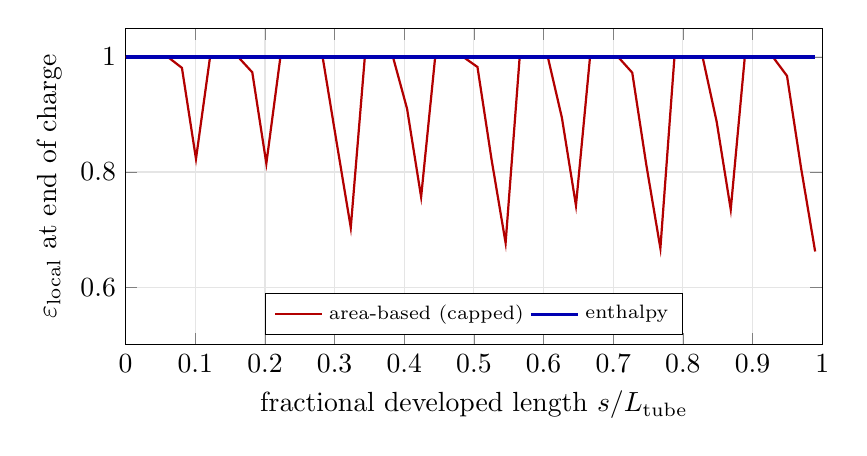
\begin{tikzpicture}
\begin{axis}[width=0.86\linewidth,height=5.6cm,
  xlabel={fractional developed length $s/L_{\mathrm{tube}}$},
  ylabel={$\varepsilon_{\mathrm{local}}$ at end of charge},
  ymin=0.5, ymax=1.05, xmin=0, xmax=1,
  legend style={font=\scriptsize,at={(0.5,0.03)},anchor=south},
  legend columns=2, grid=both, grid style={gray!20}]
\addplot[thick,red!70!black] coordinates {(0,1.0000) (0.0202,1.0000) (0.0404,1.0000) (0.06061,1.0000) (0.08081,0.9811) (0.101,0.8229) (0.1212,1.0000) (0.1414,1.0000) (0.1616,1.0000) (0.1818,0.9734) (0.202,0.8149) (0.2222,1.0000) (0.2424,1.0000) (0.2626,1.0000) (0.2828,1.0000) (0.303,0.8509) (0.3232,0.7034) (0.3434,1.0000) (0.3636,1.0000) (0.3838,1.0000) (0.404,0.9102) (0.4242,0.7567) (0.4444,1.0000) (0.4646,1.0000) (0.4848,1.0000) (0.5051,0.9826) (0.5253,0.8220) (0.5455,0.6768) (0.5657,1.0000) (0.5859,1.0000) (0.6061,1.0000) (0.6263,0.8945) (0.6465,0.7419) (0.6667,1.0000) (0.6869,1.0000) (0.7071,1.0000) (0.7273,0.9728) (0.7475,0.8124) (0.7677,0.6675) (0.7879,1.0000) (0.8081,1.0000) (0.8283,1.0000) (0.8485,0.8875) (0.8687,0.7349) (0.8889,1.0000) (0.9091,1.0000) (0.9293,1.0000) (0.9495,0.9671) (0.9697,0.8068) (0.9899,0.6619)};
\addlegendentry{area-based (capped)}
\addplot[very thick,blue!70!black] coordinates {(0,1.0000) (0.0202,1.0000) (0.0404,1.0000) (0.06061,1.0000) (0.08081,1.0000) (0.101,1.0000) (0.1212,1.0000) (0.1414,1.0000) (0.1616,1.0000) (0.1818,1.0000) (0.202,1.0000) (0.2222,1.0000) (0.2424,1.0000) (0.2626,1.0000) (0.2828,1.0000) (0.303,1.0000) (0.3232,1.0000) (0.3434,1.0000) (0.3636,1.0000) (0.3838,1.0000) (0.404,1.0000) (0.4242,1.0000) (0.4444,1.0000) (0.4646,1.0000) (0.4848,1.0000) (0.5051,1.0000) (0.5253,1.0000) (0.5455,1.0000) (0.5657,1.0000) (0.5859,1.0000) (0.6061,1.0000) (0.6263,1.0000) (0.6465,1.0000) (0.6667,1.0000) (0.6869,1.0000) (0.7071,1.0000) (0.7273,1.0000) (0.7475,1.0000) (0.7677,1.0000) (0.7879,1.0000) (0.8081,1.0000) (0.8283,1.0000) (0.8485,1.0000) (0.8687,1.0000) (0.8889,1.0000) (0.9091,1.0000) (0.9293,1.0000) (0.9495,1.0000) (0.9697,1.0000) (0.9899,1.0000)};
\addlegendentry{enthalpy}
\end{axis}
\end{tikzpicture}
\caption{Local melted fraction along the exchanger at end of charge, compared
at \emph{equal} exchanger size with the melted fraction capped in both
formulations. The sawtooth in the area-based curve is the cascade: each layer
melts fully at its inlet end and incompletely at its outlet end, because a
segment that has finished melting continues to draw heat at the full driving
difference. Under the enthalpy formulation that segment superheats instead, its
demand collapses, and the heat passes downstream --- the curve is flat at
unity. Spread falls from $0.405$ to $0.000$ (Table~\ref{tab:levelling}).}
\label{fig:levelling}
\end{figure}



\subsection{Cyclic steady state}
\label{sec:css}

The results above are \emph{first-cycle} results: the store begins fully solid
at $\Tm$ and the cycle does not return to that state. Repeating the
charge--discharge schedule drives the store to a cyclic steady state (CSS) in
which the end-of-cycle state reproduces the start-of-cycle state. Convergence
takes of order thirty cycles here.

At CSS the enthalpy change over a complete cycle is zero by definition, and the
store is adiabatic, so
\begin{equation}
  \eta_{\mathrm{storage}}(\mathrm{CSS}) \;\equiv\; 1
  \label{eq:css-unity}
\end{equation}
identically --- for every exchanger size and every flow rate; computed values
agree to eight decimal places. Equation~\eqref{eq:css-unity} is energy
conservation applied to a closed cycle rather than a result about the store, but
it has a consequence for how such a model may be posed.

\paragraph{Sizing cannot be closed on the energy balance at CSS.}
A single-cycle model sizes the exchanger by requiring that it absorb a specified
energy within the charging window. At CSS the absorbed and recovered energies
are the \emph{same number}, so that requirement and the corresponding discharge
requirement collapse into one equation. It fixes the ratio of the two flow rates
and says nothing about the exchanger size:

\begin{center}
\begin{tabular}{@{}r r r r@{}}
\toprule
$\Nwells$ & flow ratio & charge/target & discharge/target \\
\midrule
11.0 & 1.0740 & 1.00000 & 1.00000 \\
14.0 & 1.0280 & 0.99994 & 0.99994 \\
20.0 & 0.9965 & 0.99994 & 0.99994 \\
\bottomrule
\end{tabular}
\end{center}

\noindent
Adding a loss mechanism would not remove this degeneracy: at CSS the charge
would then exceed the discharge by exactly the loss, and the one remaining
equation would still pin the flow ratio.

\paragraph{Reformulation.}
The resolution is to specify the hardware and \emph{simulate} rather than solve.
The exchanger count is taken from the latent inventory alone,
$\Delta E/(\rhom V_{\mathrm{well}}\hm)$ --- a deliberate overestimate, since it
ignores the sensible capacity the store also has --- and both flows are pinned
by their specified glides. No quantity is solved for, so no convergence question
arises, and the deviation of delivered energy from target becomes a reported
result.

\begin{table}[htbp]
\centering
\caption{Cyclic steady state: deviation from target against exchanger count.
Each row is an independent march to CSS.}
\label{tab:css}
\begin{tabular}{@{}r r r r@{}}
\toprule
$\Nwells$ & delivered/target & $\varepsilon$ end charge & $\varepsilon$ end discharge \\
\midrule
11.544 & 0.9426 & 1.000 & 0.154 \\
14.000 & 0.9662 & 1.000 & 0.288 \\
16.000 & 0.9777 & 1.000 & 0.376 \\
20.000 & 0.9931 & 1.000 & 0.505 \\
26.000 & 1.0082 & 1.000 & 0.629 \\
\bottomrule
\end{tabular}
\end{table}

%---------------------------------------------------------------------
\begin{figure}[htbp]
\centering
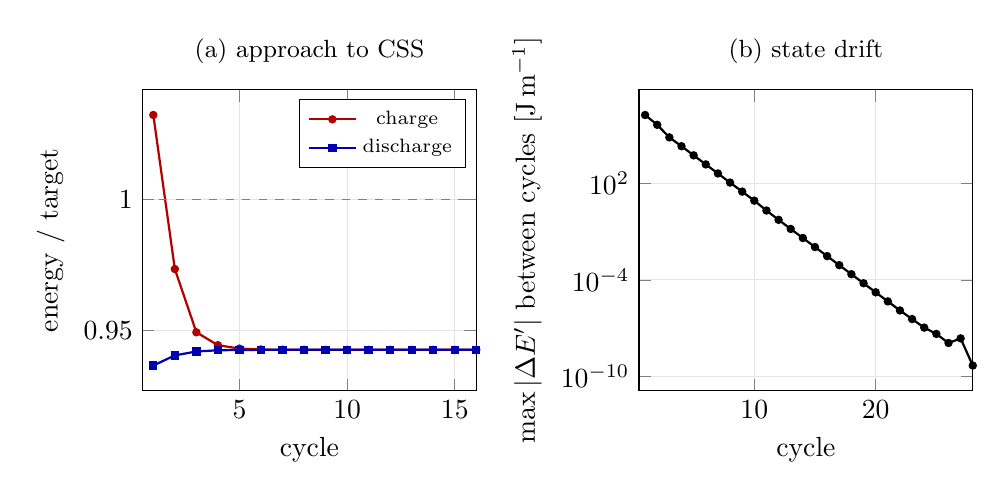
\begin{tikzpicture}
\begin{axis}[width=0.48\linewidth,height=5.4cm,
  xlabel={cycle}, ylabel={energy / target}, xmin=0.5, xmax=16,
  title={\small (a) approach to CSS},
  legend style={font=\scriptsize,at={(0.97,0.97)},anchor=north east},
  grid=both, grid style={gray!20}]
\addplot[thick,mark=*,mark size=1.1pt,red!70!black] coordinates {(1,1.03215) (2,0.97343) (3,0.94932) (4,0.94440) (5,0.94312) (6,0.94277) (7,0.94267) (8,0.94265) (9,0.94264) (10,0.94264) (11,0.94264) (12,0.94264) (13,0.94264) (14,0.94264) (15,0.94264) (16,0.94264) (17,0.94264) (18,0.94264) (19,0.94264) (20,0.94264) (21,0.94264) (22,0.94264) (23,0.94264) (24,0.94264) (25,0.94264) (26,0.94264) (27,0.94264) (28,0.94264)};
\addlegendentry{charge}
\addplot[thick,mark=square*,mark size=1.1pt,blue!70!black] coordinates {(1,0.93665) (2,0.94052) (3,0.94201) (4,0.94246) (5,0.94259) (6,0.94262) (7,0.94263) (8,0.94264) (9,0.94264) (10,0.94264) (11,0.94264) (12,0.94264) (13,0.94264) (14,0.94264) (15,0.94264) (16,0.94264) (17,0.94264) (18,0.94264) (19,0.94264) (20,0.94264) (21,0.94264) (22,0.94264) (23,0.94264) (24,0.94264) (25,0.94264) (26,0.94264) (27,0.94264) (28,0.94264)};
\addlegendentry{discharge}
\addplot[dashed,gray,domain=0.5:16,samples=2,forget plot] {1};
\end{axis}
\begin{axis}[width=0.48\linewidth,height=5.4cm,at={(0.52\linewidth,0)},
  xlabel={cycle}, ylabel={$\max|\Delta E'|$ between cycles [\si{\joule\per\meter}]},
  ymode=log, title={\small (b) state drift}, xmin=0.5, xmax=28,
  grid=both, grid style={gray!20}]
\addplot[thick,mark=*,mark size=1.1pt,black] coordinates {(1,1.8176e+06) (2,4.4441e+05) (3,7.3527e+04) (4,2.0698e+04) (5,5.5899e+03) (6,1.5284e+03) (7,4.1826e+02) (8,1.1346e+02) (9,3.1015e+01) (10,8.4881e+00) (11,2.0663e+00) (12,5.4292e-01) (13,1.4715e-01) (14,4.0183e-02) (15,1.0989e-02) (16,3.0059e-03) (17,8.2231e-04) (18,2.2496e-04) (19,6.1545e-05) (20,1.6842e-05) (21,4.5870e-06) (22,1.2470e-06) (23,3.6345e-07) (24,1.0675e-07) (25,4.3190e-08) (26,1.1758e-08) (27,2.2817e-08) (28,4.6566e-10)};
\end{axis}
\end{tikzpicture}
\caption{Convergence to cyclic steady state at the latent-only exchanger count.
(a) The first cycle is the outlier: it starts from a cold, fully solid store and
absorbs more than any later cycle. Charge and discharge converge to the
\emph{same} value, which is Eq.~\eqref{eq:css-unity} in practice --- the two
curves become indistinguishable, not merely close. (b) The state drift falls
geometrically; the run is stopped at $10^{-9}$.}
\label{fig:cssconv}
\end{figure}


Figure~\ref{fig:cssconv}(a) is worth dwelling on. The charge curve starts
\emph{above} target and falls; the discharge curve starts below and rises; they
meet. That meeting is not a numerical coincidence but
Eq.~\eqref{eq:css-unity} asserting itself: once the state repeats, the two
energies are the same number. The first cycle absorbs more than any later one
because it alone begins from a cold, fully solid store --- which is precisely
why a first-cycle result cannot be quoted for a repeating duty.

At the latent-only size the field delivers \SI{94.26}{\percent} of target. The
store melts \emph{completely} at end of charge --- $\varepsilon_{\mathrm{local}}
= 1.000$ at every station --- but returns only to a mean of $0.154$, so the
shortfall is a \textbf{discharge rate} limit rather than an inventory limit. The
signature is in the last column, drawn in Fig.~\ref{fig:cssdesign}: the residual
melt fraction \emph{rises} with exchanger count, because each unit is then
worked less hard and proportionally less of it refreezes. Were the limit an
inventory limit it would fall, since a larger store would be proportionally
emptier at the end of a fixed discharge. The two curves therefore separate the
two failure modes without any additional calculation, and they place the lever
on the discharge side --- flow rate, window length, or conductance --- rather
than on more phase-change material.
%---------------------------------------------------------------------
\begin{figure}[htbp]
\centering
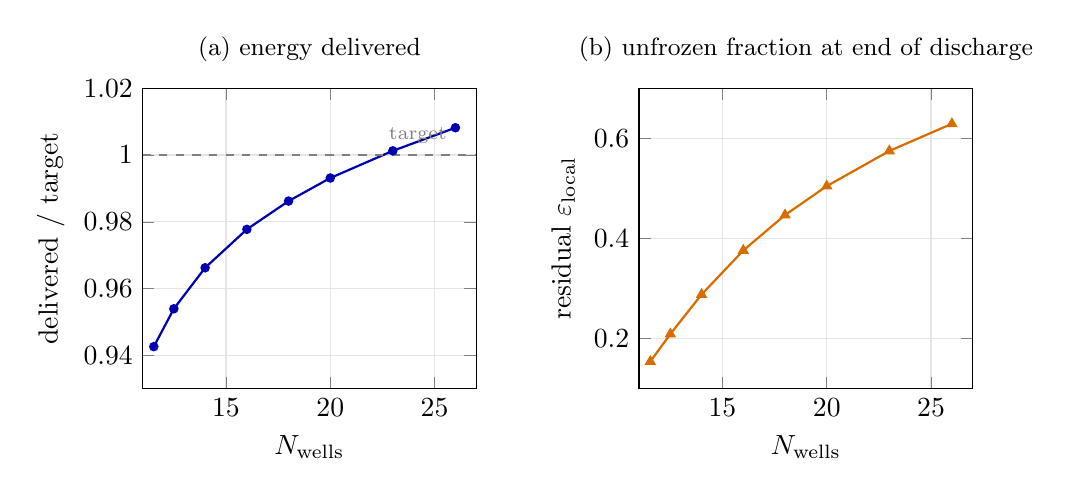
\begin{tikzpicture}
\begin{axis}[width=0.48\linewidth,height=5.4cm,
  xlabel={$\Nwells$}, ylabel={delivered / target},
  title={\small (a) energy delivered}, ymin=0.93, ymax=1.02, xmin=11, xmax=27,
  grid=both, grid style={gray!20}]
\addplot[thick,mark=*,mark size=1.3pt,blue!70!black] coordinates {(11.54,0.94264) (12.5,0.95396) (14,0.96624) (16,0.97774) (18,0.98621) (20,0.99311) (23,1.00125) (26,1.00816)};
\addplot[dashed,gray,domain=11:27,samples=2,forget plot] {1};
\node[font=\scriptsize,gray] at (axis cs:24.2,1.006) {target};
\end{axis}
\begin{axis}[width=0.48\linewidth,height=5.4cm,at={(0.52\linewidth,0)},
  xlabel={$\Nwells$},
  ylabel={residual $\varepsilon_{\mathrm{local}}$},
  title={\small (b) unfrozen fraction at end of discharge},
  ymin=0.10, ymax=0.70, xmin=11, xmax=27,
  grid=both, grid style={gray!20}]
\addplot[thick,mark=triangle*,mark size=1.6pt,orange!85!black] coordinates {(11.54,0.1545) (12.5,0.2093) (14,0.2883) (16,0.3762) (18,0.4469) (20,0.5046) (23,0.5747) (26,0.6290)};
\end{axis}
\end{tikzpicture}
\caption{Cyclic steady state against exchanger count; each point is an
independent march to convergence. (a) Delivered energy crosses target near
$\Nwells\approx23$, about twice the latent-only count. (b) The diagnostic: the
residual melted fraction at end of discharge \emph{rises} with exchanger count,
because each unit is then worked less hard and proportionally less of it
refreezes. An inventory-limited store would show the opposite, since a larger
store would be proportionally emptier after a fixed discharge. Note that the two
panels carry different quantities on similar-looking curves; they are plotted
separately for that reason.}
\label{fig:cssdesign}
\end{figure}


\subsection{Consequence for sizing}

Because the formulation conserves energy and bounds the melted fraction, the
store may be sized against two independent requirements rather than one. Writing
$\Delta E$ for the energy to be stored, the field must both \emph{absorb} it
within the charging window and \emph{contain} it at all:
\begin{equation}
  \Nwells = \max\bigl(N_{\mathrm{rate}},\,N_{\mathrm{capacity}}\bigr),
  \qquad
  N_{\mathrm{capacity}} = \frac{\Delta E}
  {\rhom V_{\mathrm{well}}\left[\hm+c_{p,l}\Delta T\right]}.
  \label{eq:sizing}
\end{equation}
$N_{\mathrm{rate}}$ follows from a root solve on the march and carries every
thermal parameter; $N_{\mathrm{capacity}}$ is closed form and carries none, which
makes it a hard lower bound no design can better. This applies to the
\emph{first} cycle; \S\ref{sec:css} shows that the rate criterion does not
survive the passage to cyclic steady state.

%=======================================================================
\section{Conclusions}
\label{sec:conclusions}

A lumped enthalpy state has been formulated for phase-change material in the
segments of a one-dimensional heat exchanger model, together with the closure
that couples it to an effectiveness--NTU march and an exact time integrator for
the resulting equation.

\begin{enumerate}[leftmargin=1.8em,itemsep=3pt]
\item Carrying enthalpy rather than melted area removes a structural defect in
  reduced-order latent storage models. A segment whose phase change is complete
  has somewhere to put further heat, so none is discarded and the melted
  fraction is confined to $[0,1]$ by the constitutive relation rather than by a
  guard. In the case examined, an area-based formulation discarded up to
  \SI{148}{\percent} of the delivered heat during discharge.
\item The conductance closing the segment equation is
  $K=\md c_{p}(1-e^{-\mathrm{NTU}})/\Delta z$ and not $\Ui P_{i}$. The two agree
  only as $\mathrm{NTU}\to0$, differ by \SI{4}{\percent} to \SI{33}{\percent}
  over the case studied, and only the former carries the capacity-rate limit
  that prevents heat flowing from cold to hot as the wall conductance improves.
\item Explicit time stepping is exact on the latent plateau and inadmissible off
  it, which is why area-based formulations never encountered the constraint. The
  branchwise-exact scheme of \S\ref{sec:integration} is unconditionally stable,
  makes energy closure structural, and agrees with a \num{200000}-substep
  reference to $3\times10^{-13}$.
\item Sensible capacity is self-levelling. Although it carries only about
  \SI{4.7}{\percent} of the energy in the case studied, it redistributes the
  melting: compared at equal exchanger size, the spread in local melted fraction
  falls from $0.405$ to $0.000$ and dead volume falls correspondingly. The
  effect is first-order in the distribution while being small in the energy,
  because it acts through the driving temperature difference rather than through
  the energy stored.
\item At cyclic steady state the recovered-to-stored energy ratio is identically
  unity in an adiabatic store (\S\ref{sec:css}), which collapses the charge and
  discharge energy requirements into a single equation. That equation fixes the
  ratio of the two flow rates and leaves the exchanger size undetermined, so a
  single-cycle sizing procedure does not carry over. Posing the problem as a
  simulation --- specify the hardware, march to CSS, report the deviation from
  target --- removes the difficulty rather than working around it, and turns the
  residual melt fraction into a diagnostic that distinguishes a rate limit from
  an inventory limit.
\end{enumerate}

\paragraph{Limitations.}
Three assumptions bound the results above and are stated here rather than left
implicit. Hypothesis H3 is \emph{saturated} at the design point: the melt fronts
of neighbouring tubes are in contact over \SI{99}{\percent} of the exchanger, so
the annular conduction resistance is evaluated at the limit of its validity and
the residual solid --- which occupies the corners between tubes, on a longer and
narrower conduction path than an annulus represents --- has its resistance
understated. Hypothesis H6 assumes the cell boundary adiabatic, which for an
axially graded store requires a physical partition between layers that are, at
the inlet end of the case studied, \SI{48.9}{\kelvin} apart; a slab estimate
places the neglected cross-boundary leak at some \SI{25}{\percent} of the useful
duty, and it flows in the direction that erodes the grading. Finally, the time
grid is not converged: $\varepsilon_{\mathrm{PCM}}$ moves $-0.3\,\%$ between
\num{40} and \num{320} time levels, one-sided. The first two are geometric
questions about a cell's outer boundary and would be settled together by a
two-dimensional conduction calculation on the real cross-section, which is the
natural next step. None of the three affects the formulation or the integrator,
which are the subject of this paper; all three affect the quantitative results
of \S\ref{sec:demo}, which should accordingly be read as optimistic. In
particular the \SI{-5.7}{\percent} cyclic-steady-state deviation of
\S\ref{sec:css} sits inside the band those three assumptions span, and is
better read as evidence that the store is discharge-rate limited than as a
calibrated shortfall.

%=======================================================================
\section*{Nomenclature}

\noindent
\begin{tabular}{@{}l l l@{}}
$\Amelt$ & melted cross-section per unit tube length & \si{\meter\squared} \\
$\Aav$ & PCM cross-section owned by one segment & \si{\meter\squared} \\
$A_{\mathrm{flow}}$ & tube flow area & \si{\meter\squared} \\
$c_{p}$ & specific heat capacity & \si{\joule\per\kilogram\per\kelvin} \\
$C_{s},C_{l}$ & sensible capacity per unit tube length & \si{\joule\per\meter\per\kelvin} \\
$E'$ & PCM enthalpy per unit tube length & \si{\joule\per\meter} \\
$\Elat$ & latent capacity per unit tube length & \si{\joule\per\meter} \\
$\Eeq$ & equilibrium enthalpy & \si{\joule\per\meter} \\
$\hm$ & latent heat of fusion & \si{\joule\per\kilogram} \\
$h_{e},h_{i}$ & outer, inner heat transfer coefficient & \si{\watt\per\meter\squared\per\kelvin} \\
$K$ & segment conductance per unit tube length & \si{\watt\per\meter\per\kelvin} \\
$\km,k_{w}$ & PCM, wall thermal conductivity & \si{\watt\per\meter\per\kelvin} \\
$L_{f},t_{f},n_{f}$ & fin length, thickness, count & \si{\meter},\si{\meter},-- \\
$\md$ & mass flow rate & \si{\kilogram\per\second} \\
$\mathrm{NTU}$ & number of transfer units per segment & -- \\
$P_{T}$ & finned outer perimeter & \si{\meter} \\
$q'$ & heat rate per unit tube length & \si{\watt\per\meter} \\
$r_{i},r_{e}$ & tube inner, outer radius & \si{\meter} \\
$s$ & developed tube coordinate & \si{\meter} \\
$\mathrm{Ste}$ & Stefan number, $c_{p}\Delta T/\hm$ & -- \\
$T$ & fluid temperature & \si{\kelvin} \\
$\Tm,\Tpcm$ & melting, PCM temperature & \si{\kelvin} \\
$\Ui$ & overall coefficient on inner area & \si{\watt\per\meter\squared\per\kelvin} \\
$\Delta z$ & segment length & \si{\meter} \\
$\delta$ & melt-layer thickness & \si{\meter} \\
$\varepsilon_{\mathrm{local}}$ & melted fraction of one segment & -- \\
$\etaf,\etao$ & fin, overall surface efficiency & -- \\
$\rhom$ & PCM density & \si{\kilogram\per\meter\cubed} \\
\end{tabular}

%=======================================================================
% NOTE. This bibliography is a STUB. The five entries below are canonical
% works that the text genuinely leans on. The application-specific
% literature -- prior wellbore-storage work, the PCM property source, and
% the author's own earlier conference paper -- still has to be added, and
% every entry should be checked against the publisher record before
% submission.
%=======================================================================
\begin{thebibliography}{9}

\bibitem{Voller1987}
V.~R. Voller, C.~Prakash,
A fixed grid numerical modelling methodology for convection-diffusion mushy
region phase-change problems,
\emph{International Journal of Heat and Mass Transfer} 30 (1987) 1709--1719.

\bibitem{Alexiades1993}
V.~Alexiades, A.~D. Solomon,
\emph{Mathematical Modeling of Melting and Freezing Processes},
Hemisphere, Washington, DC, 1993.

\bibitem{Gnielinski1976}
V.~Gnielinski,
New equations for heat and mass transfer in turbulent pipe and channel flow,
\emph{International Chemical Engineering} 16 (1976) 359--368.

\bibitem{Bell2014}
I.~H. Bell, J.~Wronski, S.~Quoilin, V.~Lemort,
Pure and pseudo-pure fluid thermophysical property evaluation and the
open-source thermophysical property library CoolProp,
\emph{Industrial \& Engineering Chemistry Research} 53 (2014) 2498--2508.

\bibitem{Incropera}
F.~P. Incropera, D.~P. DeWitt, T.~L. Bergman, A.~S. Lavine,
\emph{Fundamentals of Heat and Mass Transfer}, Wiley.

\end{thebibliography}

\end{document}
